\chapter{Methods}

\section{Robotic Platform}


\section{Signed Distance Function}


\section{Gauss-Newton Algorithm}

The \textit{Gauss-Newton} algorithm is a method for finding the optimal set of parameters $\mathbf{p}$ that minimizes the sum of squares of non-linear vector-valued objective functions $e(\cdot)$
%
\begin{equation}
\hat{\mathbf{p}} = \arg\min_{p} \sum_{i=1}^N\left[ e_i(\mathbf{p})^2\right] .
\end{equation}

The Gauss-Newton algorithm is derived from the \textit{Newton} algorithm for finding roots and extremal points which itself is based on the Taylor series expansion. The Newton method for finding extremal points of the scalar objective function $f(x)$ is an iterative procedure
%
\begin{equation}
x_{t+1} = x_t - \frac{f^{(1)}(x_t)}{f^{(2)}(x_t)}
\label{eqn:newton_minimum}
\end{equation}
%
starting at an initial state $x_0$ using the first- and second-order derivatives ($f^{(1)}$, $f^{(2)}$) of the objective function.

For finding the minimum of the function $e(\cdot)$ with respect to a parameter vector $\mathbf{p}$, the first- and second-order partial derivatives are used. In particular, the first- and second-order derivatives in \ref{eqn:newton_minimum} are replaced by the gradient $\nabla e(\mathbf{p})$ and the Hessian $\nabla^2 e(\mathbf{p})$ of the objective function $e$.
The partial derivatives of the vector-valued function $e(\cdot)$ with respect to the parameter vector $\mathbf{p}$ are aggregated in the \textit{Jacobian} matrix $J\in \mathbb{R}^{i \times j}$ with elements
%
\begin{equation}
J_{i,j} = \frac{\partial e_i(\mathbf{p})}{\partial p_j} .
\end{equation}
%
Hence,
\begin{align}
\nabla e(\mathbf{p}) &= J^\top e(\mathbf{p}) \label{eqn:gn_gradient}\\
H(e) = \nabla^2 e(\mathbf{p}) &= J^\top J +  \sum_{i=1} e_i(\mathbf{p}) \nabla^2 e_i(\mathbf{p}) \label{eqn:gn_hessian_full}.
\end{align}

For small $e$, the Hessian $H(e)$ can be approximated by
\begin{equation}
H(e) \approx J^\top J \label{eqn:gn_hessian}
\end{equation}
%
neglecting the second-order derivatives. This approximation is used in the Gauss-Newton algorithm and the parameter update step becomes
%
\begin{align}
\mathbf{p}_{t+1} &= \mathbf{p}_{t} - \Delta\mathbf{p} \\
&= \mathbf{p}_{t} - H(e)^{-1} \cdot \nabla e(\mathbf{p}) \\
&= \mathbf{p}_{t} - \left(J^\top J\right)^{-1} \cdot J^\top e(\mathbf{p}) \label{eqn:gn_param_update}.
\end{align}

The parameter update $\Delta\mathbf{p}$ is proportionally driven by the gradient of the objective function and inverse proportional by the approximation of the Hessian.


\section{Prior Information}

Prior information can be used in the Gauss-Newton algorithm by modulating the Hessian approximation and the gradient towards the desired state. This is achieved by selecting an objective function and calculating its partial derivatives with respect to the parameter vector. These partial derivatives are used in the Jacobian as shown in equations \ref{eqn:gn_gradient} and \ref{eqn:gn_hessian}.

The full parameter vector in DART consists of the 6D pose of the root frame and the $N$ joints positions:
\begin{equation}
\mathbf{p} = \begin{bmatrix}
x & y & z & \phi & \theta & \psi & | & q_1 & \cdots & q_N
\end{bmatrix}
\end{equation}

with $x$, $y$, $z$ for the translation, $\phi$, $\theta$, $\psi$ for the orientation in radiant Euler angles, and $q_1 \dots q_N$ the individual joint position values.


\subsection{Known Frame Pose}

For constraining the translation of the root frame in between optimization iterations, the parameter update vector $\Delta\mathbf{p}$ must be computed such that its first 6 elements for the pose are $0$. From equation \ref{eqn:gn_param_update}
\begin{align}
\Delta\mathbf{p} &= \left(J^\top J\right)^{-1} \cdot J^\top e(\mathbf{p}) = \begin{bmatrix}
\mathbf{0} & | & q_1 & \cdots & q_N
\end{bmatrix} \\
J^\top e &= J^\top J \cdot \begin{bmatrix}
\mathbf{0} & | & q_1 & \cdots & q_N
\end{bmatrix}
\end{align}

Cancelling out the pose update can be achieved by applying the prior on the final blended Hessian and gradient just before the final parameter update is computed. In particular the fixed frame prior computes the parameter update $\Delta\mathbf{p}$ from the blended Hessian and gradient, cancels out the first 6 elements for the pose, and computes the new gradient. Instead of blending this gradient ($J^\top e$) into the final gradient, the global gradient is overwritten resulting in enforcing no frame pose update.


\subsection{Reported Joint Positions}

We use the reported state of the robot in a way, that we can drag the estimated solution away from possibly distracting perceptions towards the state perceived through the joint encoders.
%
Three different kind of objective functions have been selected for this purpose which compute a weighted deviation of the estimated joint configuration $\mathbf{q}$ from reported joint configuration $\mathbf{r}$. For all objective functions, $r_i$ and $q_i$ denote the individual joint positions in their corresponding configuration vector.

\begin{enumerate}
\item Weighted L2 norm of the estimated joint position deviation:
\begin{equation}
e_1 = w \cdot \lVert \mathbf{r} - \mathbf{q} \rVert = w \cdot \sqrt{\sum_{i=1}^N (r_i - q_i)^2} \label{eqn:objf_weightedL2}
\end{equation}
with scalar weight $w>0$.

\item L2 norm of the weighted joint deviation:
\begin{equation}
e_2 = \lVert w \cdot (\mathbf{r} - \mathbf{q}) \rVert = \sqrt{\sum_{i=1}^N w \cdot (r_i - q_i)^2} \label{eqn:objf_L2ofweighted}
\end{equation}
with the same scalar weight $w>0$ for all joint deviations.

\item Sum of squares of individually weighted joints:
\begin{equation}
e_3 = \lvert \mathbf{r} - \mathbf{q} \rvert^\top Q \lvert \mathbf{r} - \mathbf{q} \rvert = \sum_{i=1}^N \left[ (r_i-q_i) \cdot \sum_{j=1}^N (r_j-q_j) \cdot \omega_{i,j} \right] \label{eqn:objf_indiv_weighted}
\end{equation}
with the weight matrix $Q\in\mathbf{R}^{N\times N}$ and its elements $\omega_{i,j}$. As a error metric, the weight matrix $Q$ must be \emph{positive-semidefinite}. That is, $\forall \mathbf{x}\in\mathbf{R}^n: x^\top Q x \geq 0$.
\end{enumerate}

Whereas the first two objective functions (\ref{eqn:objf_weightedL2} and \ref{eqn:objf_L2ofweighted}) use a common scalar weight for all joint deviations, the third objective function (\ref{eqn:objf_indiv_weighted}) can apply different weights per joint and hence enables to penalize whole parts of the kinematic chain more precise.

The respective partial derivatives for the Jacobian are:
\begin{enumerate}
\item Weighted L2 norm of the estimated joint position deviation
\begin{equation}
J_{ji} = \frac{\partial e_1}{\partial q_i} = -w \frac{r_i - q_i}{\lVert \mathbf{r} - \mathbf{q} \rVert}
\end{equation}

\item L2 norm of the weighted joint deviation:
\begin{equation}
J_{ji} = \frac{\partial e_2}{\partial q_i} = -w^2 \frac{r_i - q_i}{\lVert w \cdot (\mathbf{r} - \mathbf{q}) \rVert}
\end{equation}

\item Sum of squares of individually weighted joints:
\begin{equation}
J_{ji} = \frac{\partial e_3}{\partial q_i} = - \left[ \sum_{j=1}^N d_jq_{i,j}\right] + \left[ \sum_{j=1 \neq i}^N d_jq_{j,i}\right]
\end{equation}
\end{enumerate}


\section{Ground Truth Data Collection}

To evaluate the tracking performance and verify the effect of the joint position prior, reference measurements of the true state of the robot are required. The Vicon motion caption system is selected to externally track the pose of IR reflective markers rigidly attached to the robot.

\subsection{Setup}

To obtain the true transformation from the pelvis frame to the left hand palm frame, reflective markers are rigidly mounted with standoffs to the specific robot frames. The photograph in \cref{fig:vicon_marker} shows the highlighted location of the markers on the \texttt{pelvis} frame (green) and the \texttt{leftPalm} frame (red).

\begin{figure}
\captionsetup{width=0.4\textwidth}
\centering
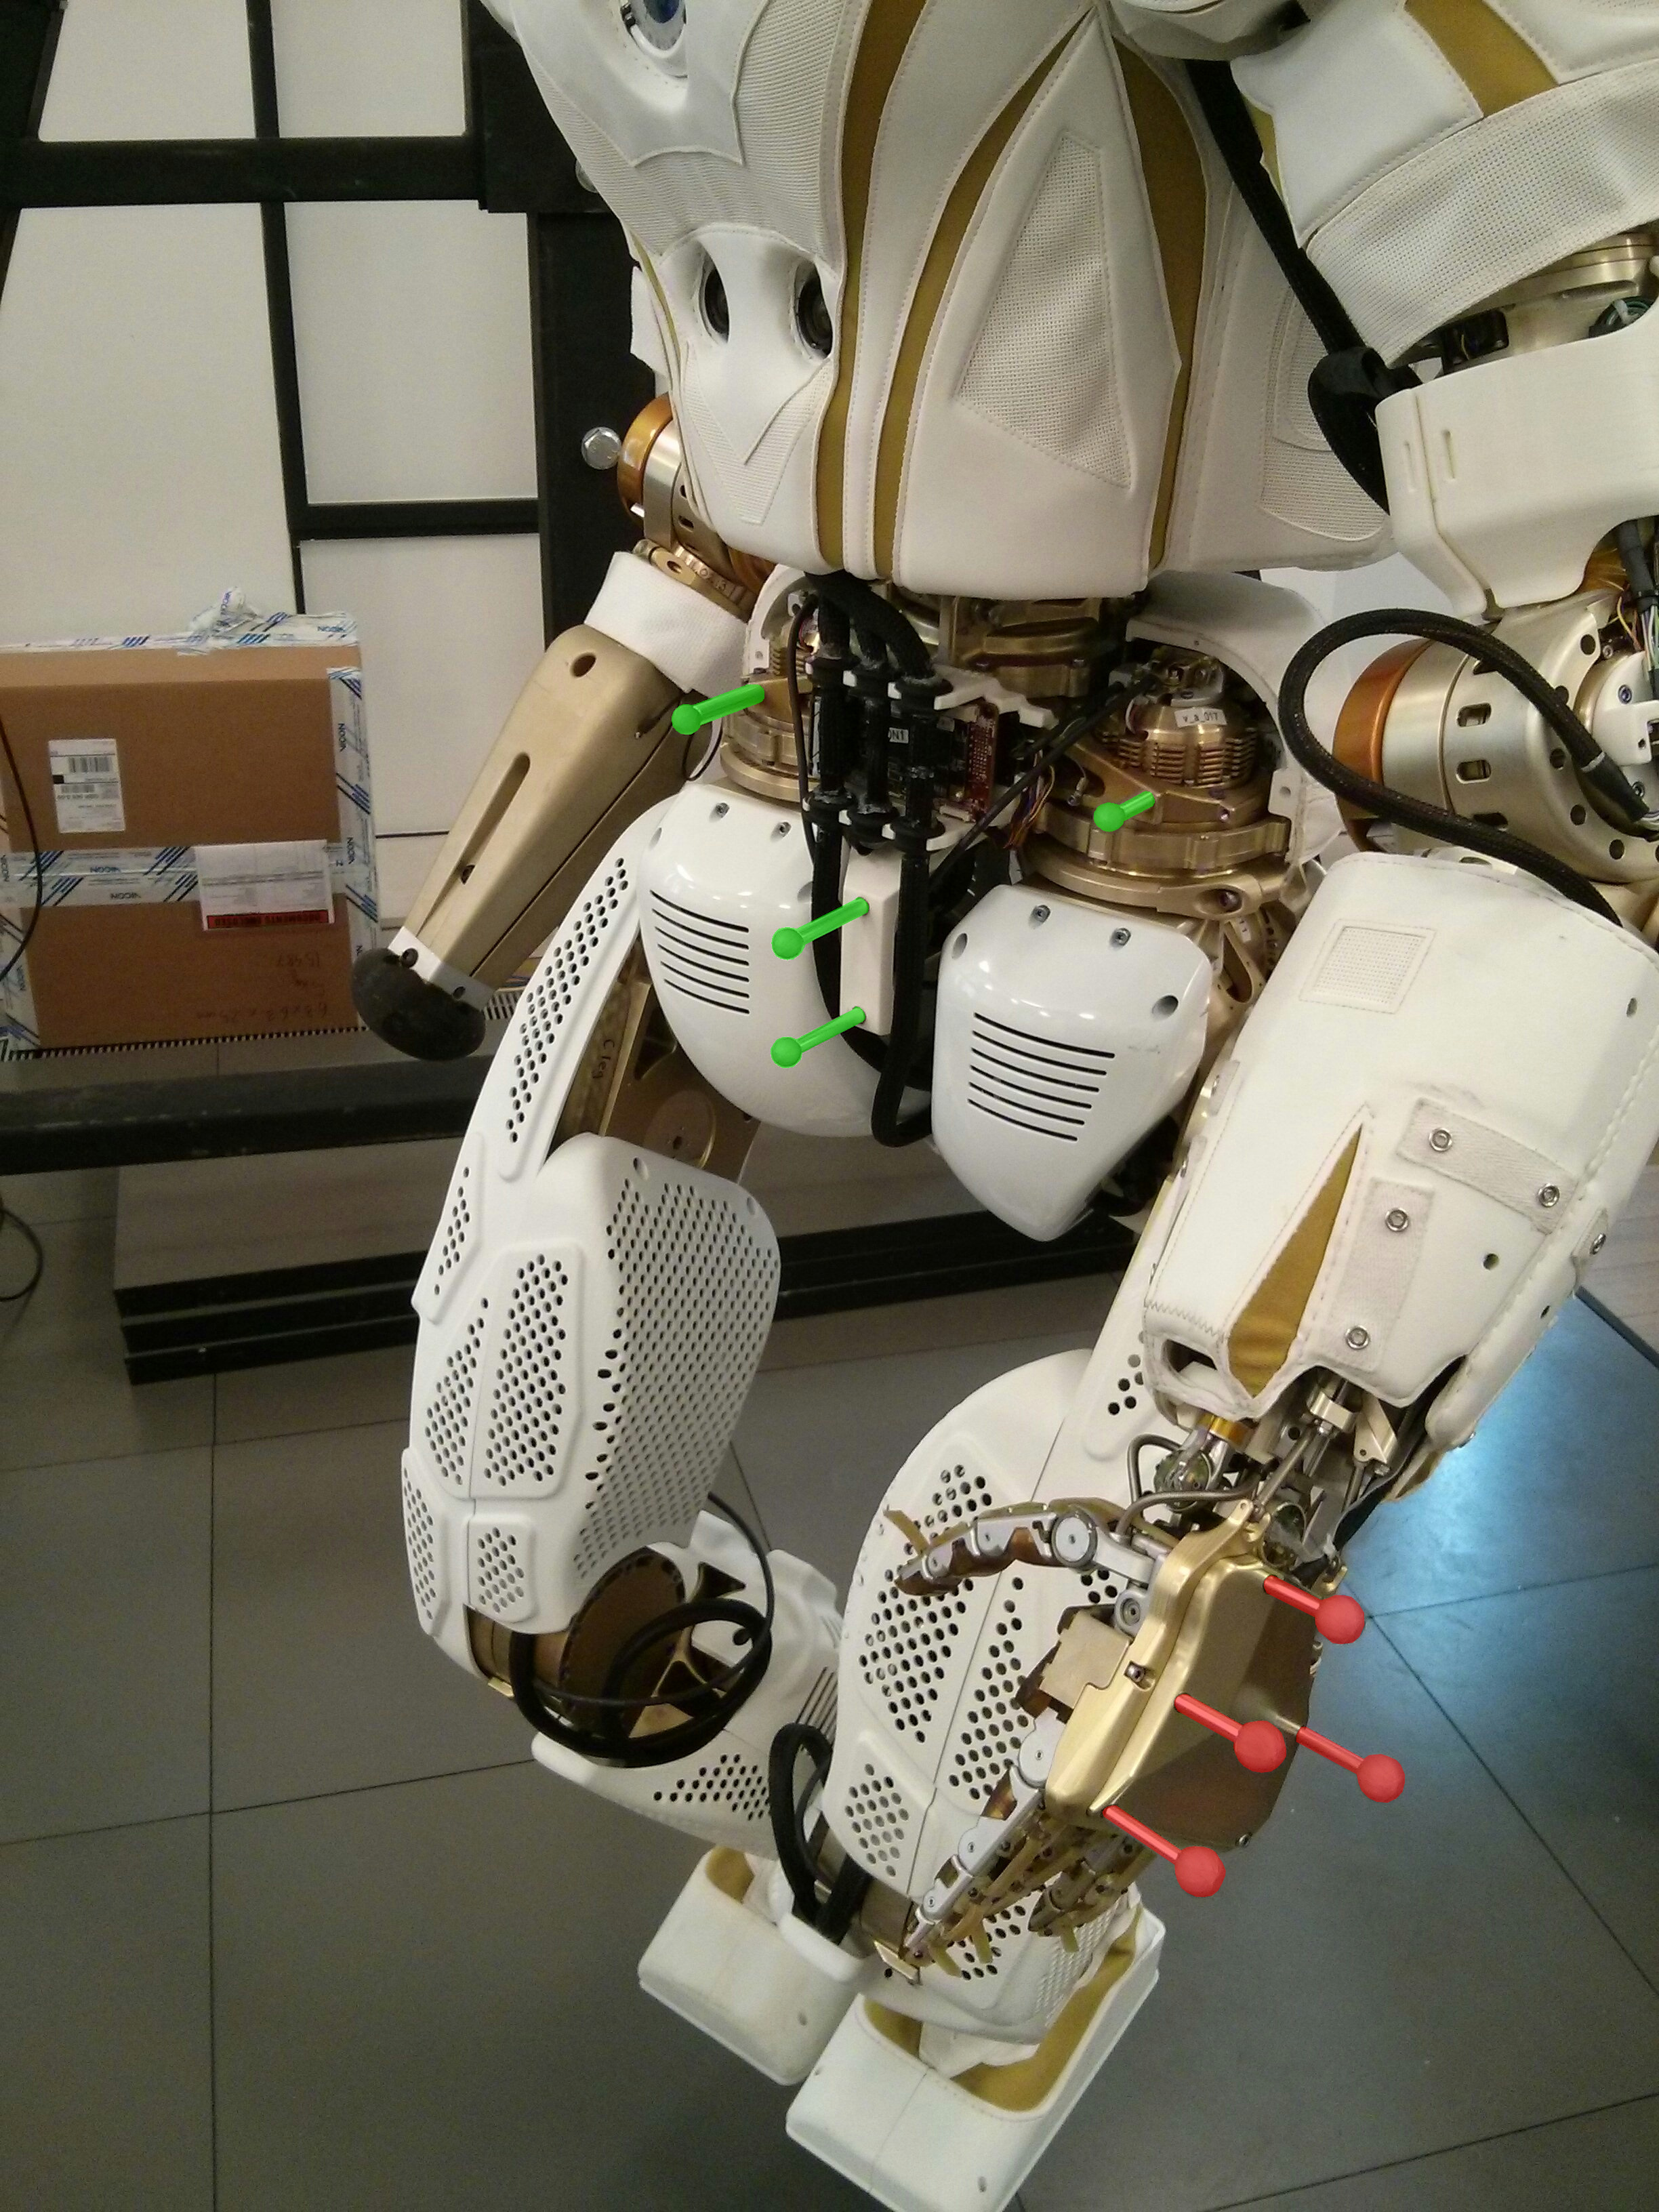
\includegraphics[width=0.4\textwidth]{images/vicon_pose/vicon_marker_col.jpg}
\caption{Location of Vicon marker on pelvis (green) and left hand (red)}
\label{fig:vicon_marker}
\end{figure}


\subsection{Hand Pose}

Each group of markers has its own coordinate system with its origin in the centre.
The drawing in \cref{fig:transform_vicon_robot} visualizes the transformations between the Vicon world frame, the Vicon marker frames and the robot frames.
The transformations $T_{w \rightarrow vp}$ and $T_{w \rightarrow vh}$ are the reported poses of the Vicon marker in the world frame.
To obtain the transformation $T_{p \rightarrow h}$, which gives the hand pose in the pelvis frame, we need to find the rigid transformation between the Vicon marker and robot frame ($T_{m \rightarrow p}$ and $T_{m \rightarrow h}$).

\begin{figure}
\captionsetup{width=0.52\textwidth}
\centering
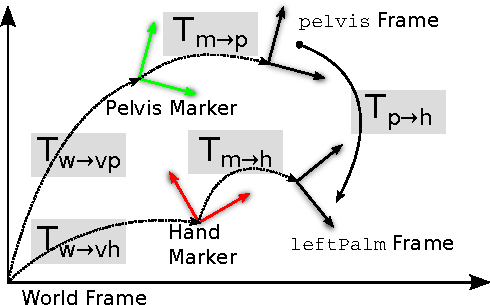
\includegraphics[width=0.5\textwidth]{images/vicon_pose/vicon_transforms.pdf}
\caption{Transformations between Vicon markers (\textit{pelvis} - green, \textit{hand} - red) and robot frames}
\label{fig:transform_vicon_robot}
\end{figure}

The rigid transformation between marker and robot frames can be obtained by a least-squares optimization on corresponding points in both frames \cite{Umeyama1991}. Given corresponding points $m_i$ in marker frame and $x_i$ in the robot frame, the optimal projection of marker points from the marker frame into corresponding points in the robot frame becomes
\begin{equation}
T_{x \rightarrow m} = \arg\min_{R,t} \frac{1}{N} \sum_{i=1}^N \lVert x_i - \left( R \cdot m_i + t \right) \rVert_2
\label{eqn:least_squares_transformation_estimation}
\end{equation}
where $T_{x \rightarrow m}$ denotes the homogeneous transformation matrix containing the rotation matrix $R$ and the translation vector $t$. The points $x_i$ in the robot frame are here interchangeable for points $p_i$ in the \texttt{pelvis} frame and $h_i$ in the \texttt{leftPalm} frame.

%The Vicon system provides the pose of the marker frame in the world coordinate frame. That is the inverse of the transformations $T_{w \rightarrow vp}^{-1}$ and $T_{w \rightarrow vh}^{-1}$, e.g. the projection of the marker into the world frame.
The pose of the \texttt{pelvis} and \texttt{leftPalm} frame in the Vicon world frame can be expressed by the transformations
\begin{align}
T_{w \rightarrow p} &= T_{w \rightarrow vp} \cdot T_{p \rightarrow m} = T_{w \rightarrow vp} \cdot T_{m \rightarrow p}^{-1} \\
T_{w \rightarrow h} &= T_{w \rightarrow vh} \cdot T_{h \rightarrow m} = T_{w \rightarrow vh} \cdot T_{m \rightarrow h}^{-1} .
\end{align}

The transformations between these robot frames then finally becomes
\begin{align}
T_{w \rightarrow h} &= T_{w \rightarrow p} \cdot T_{p \rightarrow h} \\
T_{w \rightarrow vh} \cdot T_{m \rightarrow h}^{-1} &= T_{w \rightarrow vp} \cdot T_{m \rightarrow p}^{-1} \cdot T_{p \rightarrow h} \nonumber \\
T_{p \rightarrow h} &= \left( T_{w \rightarrow vp} \cdot T_{m \rightarrow p}^{-1} \right)^{-1} \cdot T_{w \rightarrow vh} \cdot T_{m \rightarrow h}^{-1} \label{eqn:hand_pose_from_vicon} .
\end{align}

Given the transformations of the Vicon markers ($T_{w \rightarrow vp}$ and $T_{w \rightarrow vh}$) at each time instance, and the rigid transformation between these markers and the robot frame ($T_{m \rightarrow p}$ and $T_{m \rightarrow h}$) we can recover the true pose of the hand in the pelvis frame ($T_{p \rightarrow h}$) using \cref{eqn:hand_pose_from_vicon}.


\subsection{Joint Position Offsets}
